%% ============================================================
%%  Battery-Buffered EV Charging Station — Lecture Slides
%% ============================================================
\documentclass[aspectratio=169]{beamer}

\usepackage[utf8]{inputenc}
\usepackage{amsmath}
\usepackage{graphicx}
\usepackage[T1]{fontenc}
\usepackage{libertine}
\usepackage{array}
\usepackage{marvosym}
\usepackage{bm}
\usepackage{booktabs}
\usepackage{xcolor}

\usepackage{pgfplots}
\usepackage{tikz}
\usetikzlibrary{automata, arrows, positioning, calc, babel, backgrounds, matrix, shapes, shadings}
\usepgfplotslibrary{fillbetween}

\usepackage[square,authoryear]{natbib}
\renewcommand{\cite}{\citep}
\renewcommand{\bibfont}{\small}
\bibliographystyle{abbrvnat}

\newcommand{\R}{\mathbb{R}}
\newcommand{\brackets}[2]{\left\langle#1,#2\right\rangle}
\newcommand{\ind}[1]{\mathbf{1}_{\left\{#1\right\}}}
\newcommand{\mgs}{M_Y}
\newcommand{\fhat}{\hat{f}_0}
\newcommand{\graphheight}{7cm}
\newcommand{\graphwidth}{11cm}
\newcommand{\E}[1]{E\left[#1\right]}
\renewcommand{\phi}{\varphi}

\definecolor{azulcito}{RGB}{0,90,150}
\definecolor{verdecito}{RGB}{90,150,0}
\definecolor{rojito}{RGB}{150,0,90}
\definecolor{violetita}{RGB}{150,20,150}

\setbeamercolor*{structure}{fg=azulcito,bg=azulcito!20!white}
\setbeamercolor*{alerted text}{fg=azulcito}
\setbeamercolor{block title}{fg=azulcito,bg=azulcito!20!white}
\setbeamercolor{block body}{fg=black,bg=azulcito!10!white}

\beamertemplatenavigationsymbolsempty

\setbeamercolor*{author in head/foot}{fg=azulcito,bg=azulcito!15!white}
\setbeamercolor*{title in head/foot}{fg=azulcito,bg=azulcito!15!white}
\setbeamercolor*{date in head/foot}{fg=azulcito,bg=azulcito!15!white}

\pgfplotsset{width=\graphwidth, height=\graphheight, grid style={dashed,gray},
  every tick label/.append style={font=\footnotesize}, compat=1.18,
  legend style={font=\footnotesize,draw=none,fill=none},
  every axis/.append style={label style={font=\footnotesize}}}

\tikzset{>=stealth}

\newtheorem{proposition}{Proposition}
\newtheorem{remark}{Remark}

\defbeamertemplate*{footline}{mitema}{
  \leavevmode
  \hbox{%
  \begin{beamercolorbox}[wd=.25\paperwidth,ht=2.25ex,dp=1ex,left]{author in head/foot}%
    \usebeamerfont{author in head/foot}\hspace*{2ex}\insertshortauthor
  \end{beamercolorbox}%
  \begin{beamercolorbox}[wd=.5\paperwidth,ht=2.25ex,dp=1ex,center]{title in head/foot}%
    \usebeamerfont{date in head/foot}\insertshortdate{}
  \end{beamercolorbox}%
  \begin{beamercolorbox}[wd=.25\paperwidth,ht=2.25ex,dp=1ex,right]{date in head/foot}%
    \insertframenumber{}/\inserttotalframenumber\hspace*{2em}
  \end{beamercolorbox}}%
  \vskip0pt%
}

\setbeamercolor{blocky}{fg=azulcito,bg=azulcito!15!white}
\setbeamercolor{blocky2}{fg=black,bg=azulcito!10!white}

\defbeamertemplate*{title page}{customized}[1][]{
{\flushright
  \begin{beamercolorbox}[wd=\paperwidth,sep=1em,right,rightskip=1.5em]{blocky}%
    \usebeamerfont{title}{\huge \inserttitle}\par \bigskip
    \usebeamerfont{subtitle}{\large \insertsubtitle}\par
  \end{beamercolorbox}%
  \vfill
    \usebeamerfont{author}{\Large \insertauthor}\par \vspace{1em}
      \usebeamerfont{institute}{\large \insertinstitute}\par
  \vfill
  \usebeamerfont{date}{\insertdate}\par
}}

\usefonttheme[onlymath]{serif}

%% ============================================================
\title[Battery-Buffered EV Charging]{%
  Stationary Analysis of a Battery-Buffered EV Charging Station}
\subtitle{A Piecewise-Deterministic Approach}

\author[A. Ferragut]{Andres Ferragut}
\institute[Universidad ORT Uruguay]{Universidad ORT Uruguay}
\date{}

%% ============================================================
\begin{document}

\begin{frame}[plain]
  \titlepage
\end{frame}

%% ============================================================
\begin{frame}{Outline}
  \tableofcontents
\end{frame}

%% ============================================================
%% PART 1 — MOTIVATION AND PHYSICAL SETUP
%% ============================================================
\section{System Model}

%% --- Slide 1 ---
\begin{frame}{Why Battery-Buffered Charging?}

  \begin{columns}
    \begin{column}{0.55\textwidth}
      \begin{itemize}
        \setlength\itemsep{1em}
        \item Fast EV charging requires high peak power from the grid
        \item Grid connection is limited — upgrading is costly
        \item A \textbf{battery buffer} absorbs excess demand
        \item Charges slowly from the grid, discharges fast to the car
      \end{itemize}
    \end{column}
    \begin{column}{0.42\textwidth}
      \begin{center}
      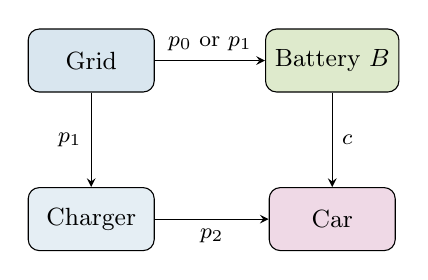
\begin{tikzpicture}[node distance=1.2cm, every node/.style={font=\small}]
        \node[draw, rounded corners, fill=azulcito!15, minimum width=1.6cm, minimum height=0.8cm] (grid) {Grid};
        \node[draw, rounded corners, fill=verdecito!20, minimum width=1.6cm, minimum height=0.8cm, right=1.4cm of grid] (bat) {Battery $B$};
        \node[draw, rounded corners, fill=rojito!15, minimum width=1.6cm, minimum height=0.8cm, below=1.2cm of bat] (car) {Car};
        \node[draw, rounded corners, fill=azulcito!10, minimum width=1.6cm, minimum height=0.8cm, below=1.2cm of grid] (charger) {Charger};

        \draw[->] (grid) -- node[above, font=\footnotesize]{$p_0$ or $p_1$} (bat);
        \draw[->] (bat) -- node[right, font=\footnotesize]{$c$} (car);
        \draw[->] (grid) -- node[left, font=\footnotesize]{$p_1$} (charger);
        \draw[->] (charger) -- node[below, font=\footnotesize]{$p_2$} (car);
      \end{tikzpicture}
      \end{center}
    \end{column}
  \end{columns}

\end{frame}

%% --- Slide 2 ---
\begin{frame}{Charging Rates}

  \begin{itemize}
    \setlength\itemsep{1em}
    \item $p_0 \leq p_1$ \quad grid-to-battery charge rate when idle\\
          {\small kept below $p_1$ to extend battery life}
    \item $p_1$ \quad grid rate when a car is present and battery is empty
    \item $p_2 > p_1$ \quad fast charging rate when battery is positive
    \item $c = p_2 - p_1$ \quad net battery discharge rate during fast charging
    \item $B$ \quad battery capacity
  \end{itemize}

  \medskip
  \begin{block}{}
    Ordering: $p_0 \leq p_1 < p_2$, so $c > 0$.
  \end{block}

\end{frame}

%%  --- Slide 3 ---
\begin{frame}{Customers and Service}

  \begin{itemize}
    \setlength\itemsep{1em}
    \item Cars arrive as a \textbf{Poisson process} of rate $\lambda$
    \item Each car has an energy demand $Y \sim F$, mean $1/\mu$
    \item \textbf{Loss system}: a car arriving when the charger is busy is turned away
  \end{itemize}

  \bigskip
  \begin{block}{Two-phase service}
    \begin{itemize}
      \setlength\itemsep{0.5em}
      \item \textbf{Phase 1} --- battery positive ($x>0$): car charges at rate $p_2$, battery depletes at rate $c$
      \item \textbf{Phase 2} --- battery empty ($x=0$): car charges at rate $p_1$, battery stays at $0$
    \end{itemize}
  \end{block}

\end{frame}

%% ============================================================
%% PART 2 — THE PDMP FORMULATION
%% ============================================================
\section{The PDMP Formulation}

%% --- Slide 4 ---
\begin{frame}{Piecewise-Deterministic Markov Processes}

  A PDMP \citep{Davis1984} is defined by three local characteristics:

  \medskip
  \begin{description}
    \setlength\itemsep{0.8em}
    \item[\normalfont Flow $r(x)$:] deterministic ODE $\dot{x} = r(x)$ between jumps
    \item[\normalfont Jump rate $\lambda(x)$:] spontaneous jumps occur at rate $\lambda(x)$
    \item[\normalfont Kernel $Q(\cdot\,;x)$:] post-jump location given pre-jump state $x$
  \end{description}

  \medskip
  \begin{block}{}
    Between jumps the process follows a deterministic trajectory.\\
    At jump times it relocates randomly according to $Q$.
  \end{block}

\end{frame}

%% --- Slide 4a ---
\begin{frame}{State Space}

  \textbf{State:} $Z(t) = (n(t),\, x(t)) \in \{0,1\} \times [0,B]$

  \bigskip
  \begin{description}
    \setlength\itemsep{1em}
    \item[$n=0$] charger idle — battery recharges from the grid
    \item[$n=1$] car being served — battery discharges (if $x>0$)
    \item[$x$] battery level — continuous, bounded in $[0,B]$
  \end{description}

  \bigskip
  \begin{block}{}
    Between jumps, $x(t)$ evolves deterministically according to $\dot{x} = r(n,x)$.\\
    Jumps occur at Poisson-like times and flip $n$.
  \end{block}

\end{frame}

%% --- Slide 4b ---
\begin{frame}{The Vector Field}

  \begin{center}
  \renewcommand{\arraystretch}{1.5}
  \begin{tabular}{ccl}
    \toprule
    $n$ & condition & $\dot{x} = r(n,x)$ \\
    \midrule
    $0$ & $x < B$ & $+p_0$ \quad (battery charges) \\
    $0$ & $x = B$ & $\phantom{+}0$ \quad (battery full, stays) \\
    $1$ & $x > 0$ & $-c$ \quad (battery discharges) \\
    $1$ & $x = 0$ & $\phantom{+}0$ \quad (battery empty, stays) \\
    \bottomrule
  \end{tabular}
  \end{center}

  \bigskip
  Setting $r=0$ at the boundaries avoids forced jumps.

  \medskip
  \textit{Cost:} we lose Lipschitz continuity at $x=0$ and $x=B$.

  \medskip
  \textit{Fix:} uniqueness via a monotonicity argument — next slide.

\end{frame}

%% --- Slide 5 ---
\begin{frame}{Well-Posedness of the Flow}

  \textbf{Question:} does $\dot{x} = r(n,x)$ have a unique solution without Lipschitz?

  \bigskip
  \begin{block}{Uniqueness via Monotonicity}
    If $r(n,\cdot)$ is \emph{non-increasing}, then the ODE has at most one solution.
    \medskip

    \textit{Proof sketch:} Let $d(t) = x(t) - y(t)$ for two solutions. Then
    \[
      \tfrac{d}{dt}\, d(t)^2 = 2\,d(t)\,[r(n,x(t)) - r(n,y(t))] \leq 0
    \]
    since $r$ is non-increasing. With $d(0)=0$ this gives $d(t)=0$ for all $t\geq 0$.
  \end{block}

  \bigskip
  In our model $r(0,\cdot)$ drops from $p_0$ to $0$ at $x=B$, and $r(1,\cdot)$ drops from $-c$ to $0$ at $x=0$ — both non-increasing. Existence follows from Carathéodory.

\end{frame}

%% --- Slide 6 ---
\begin{frame}{Jumps and Generator}

  \textbf{Spontaneous jumps only} (no forced boundary jumps):

  \medskip
  \begin{itemize}
    \setlength\itemsep{0.6em}
    \item Arrival at $(0,x)$: rate $\lambda$, flip $n\!:\, 0\to 1$, $x$ unchanged
    \item Departure at $(1,x)$, $x>0$: rate $\mu p_2$, flip $n\!:\, 1\to 0$, $x$ unchanged
    \item Departure at $(1,0)$: rate $\mu p_1$, flip $n\!:\, 1\to 0$
  \end{itemize}

  \bigskip
  \textbf{Generator} $\mathcal{A}$ acting on test functions $\psi$:
  \begin{align*}
    \mathcal{A}\psi(0,x) &= r(0,x)\,\psi_0'(x) + \lambda\,[\psi(1,x) - \psi(0,x)] \\
    \mathcal{A}\psi(1,x) &= r(1,x)\,\psi_1'(x) + \mu p(x)\,[\psi(0,x) - \psi(1,x)]
  \end{align*}
  where $p(x) = p_2\,\mathbf{1}_{x>0} + p_1\,\mathbf{1}_{x=0}$.

\end{frame}

%% ============================================================
%% PART 3 — STATIONARY DISTRIBUTION: EXPONENTIAL DEMANDS
%% ============================================================
\section{Exponential Demands}

%% --- Slide 7 ---
\begin{frame}{Structure of the Stationary Distribution}

  The stationary distribution $\pi$ has a \textbf{mixed} structure:

  \bigskip
  \begin{center}
  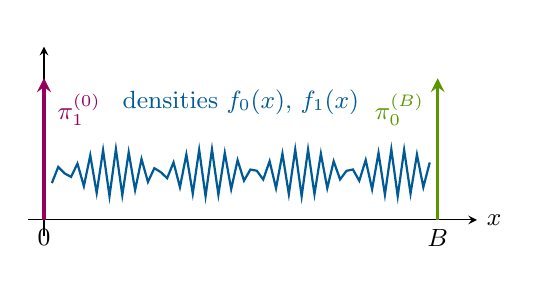
\begin{tikzpicture}[scale=1.0, font=\small]
    % x-axis
    \draw[->] (-0.2,0) -- (5.5,0) node[right]{$x$};
    \draw[->] (0,-0.2) -- (0,2.2) node[above]{};
    % labels on x-axis
    \node[below] at (0,0) {$0$};
    \node[below] at (5,0) {$B$};
    % densities label
    \node[azulcito] at (2.5,1.5) {densities $f_0(x),\, f_1(x)$};
    % atom at 0
    \draw[rojito, very thick, ->] (0,0) -- (0,1.8);
    \node[rojito, right] at (0.05,1.4) {$\pi_1^{(0)}$};
    % atom at B
    \draw[verdecito, very thick, ->] (5,0) -- (5,1.8);
    \node[verdecito, left] at (4.95,1.4) {$\pi_0^{(B)}$};
    % wavy line for densities
    \draw[azulcito, thick, domain=0.1:4.9, samples=60]
      plot(\x, {0.6 + 0.3*sin(180*\x/5 r)});
  \end{tikzpicture}
  \end{center}

  \medskip
  \begin{itemize}
    \item $\pi_1^{(0)}$: probability of battery empty, car being served
    \item $\pi_0^{(B)}$: probability of battery full, charger idle
    \item No mass at $(0,0)$: battery always positive at arrivals (Poisson)
  \end{itemize}

\end{frame}

%% --- Slide 8 ---
\begin{frame}{Kolmogorov Forward Equations}

  Setting $\partial/\partial t = 0$ in the forward equation gives the \textbf{interior balance}:

  \begin{align}
    p_0\, f_0'(x) &= -\lambda\, f_0(x) + \mu p_2\, f_1(x) \tag{E0} \\[4pt]
    -c\, f_1'(x) &= \lambda\, f_0(x) - \mu p_2\, f_1(x) \tag{E1}
  \end{align}

  \bigskip
  \textbf{Boundary flux balance} at $x=0$ and $x=B$:
  \begin{align*}
    p_0\, f_0(0^+) &= c\, f_1(0^+) = \mu p_1\, \pi_1^{(0)} \\[4pt]
    p_0\, f_0(B^-) &= c\, f_1(B^-) = \lambda\, \pi_0^{(B)}
  \end{align*}

  \medskip
  Each equation says: \emph{probability flux in = probability flux out}.

\end{frame}

%% --- Slide 9 ---
\begin{frame}{Proportionality and the Key ODE}

  \textbf{Step 1.} Add (E0) and (E1):
  \[
    \frac{d}{dx}\bigl[p_0\,f_0(x) - c\,f_1(x)\bigr] = 0
  \]
  So $p_0 f_0 - c f_1 = \text{const}$. The boundary condition at $x=0$ gives const $= 0$:
  \[
    \boxed{f_1(x) = \frac{p_0}{c}\,f_0(x)}
  \]

  \bigskip
  \textbf{Step 2.} Substitute into (E0):
  \[
    f_0'(x) = \underbrace{\left(\frac{\mu p_2}{c} - \frac{\lambda}{p_0}\right)}_{\displaystyle\theta_1} f_0(x)
  \]

  The solution is $f_0(x) = f_0(0^+)\,e^{\theta_1 x}$.

\end{frame}

%% --- Slide 10 ---
\begin{frame}{Physical Meaning of $\theta_1$}

  Consider the battery level \emph{without} the constraints at $0$ and $B$:

  \medskip
  \begin{itemize}
    \setlength\itemsep{0.6em}
    \item Battery charges at rate $p_0$ when idle (fraction of time $\approx \mu p_2/(\lambda+\mu p_2)$)
    \item Battery drains at rate $c$ when busy (fraction of time $\approx \lambda/(\lambda+\mu p_2)$)
  \end{itemize}

  \medskip
  The \textbf{mean drift} of the unconstrained battery is proportional to:
  \[
    \theta_1 = \frac{\mu p_2}{c} - \frac{\lambda}{p_0}
  \]

  \bigskip
  \begin{center}
  \renewcommand{\arraystretch}{1.3}
  \begin{tabular}{cl}
    \toprule
    $\theta_1 > 0$ & battery drifts up — station lightly loaded \\
    $\theta_1 = 0$ & critical balance — uniform density \\
    $\theta_1 < 0$ & battery drifts down — station heavily loaded \\
    \bottomrule
  \end{tabular}
  \end{center}

\end{frame}

%% --- Slide 11 ---
\begin{frame}{Complete Solution}

  \[
    f_0(x) = \frac{e^{\theta_1 x}}{K}, \qquad
    f_1(x) = \frac{p_0}{c}\cdot\frac{e^{\theta_1 x}}{K}, \qquad x\in(0,B)
  \]
  \[
    \pi_1^{(0)} = \frac{p_0}{\mu p_1 K}, \qquad
    \pi_0^{(B)} = \frac{p_0}{\lambda K}\,e^{\theta_1 B}
  \]

  \medskip
  Normalization constant:
  \[
    K = \frac{p_0+c}{c}\cdot\frac{e^{\theta_1 B}-1}{\theta_1}
      + \frac{p_0}{\mu p_1} + \frac{p_0}{\lambda}\,e^{\theta_1 B}
  \]

\end{frame}

%% --- Slide 11b ---
\begin{frame}{A Key Structural Result}

  \begin{block}{Decoupling in the interior}
    The battery level and the charger occupancy are independent given $x\in(0,B)$:
    \[
      \Pr(n=1 \mid x) = \frac{p_0}{p_0+c} \qquad \text{for all } x\in(0,B)
    \]
  \end{block}

  \bigskip
  Knowing the battery level gives no information about whether a car is being served.

\end{frame}

%% --- Slide 12 ---
\begin{frame}{Performance Metrics}

  \renewcommand{\arraystretch}{1.5}
  \begin{tabular}{lll}
    \toprule
    Metric & Formula & Limit $B\to\infty$ \\
    \midrule
    Blocking $P_B$ &
      $\dfrac{p_0}{K}\!\left(\dfrac{e^{\theta_1 B}-1}{c\,\theta_1}+\dfrac{1}{\mu p_1}\right)$ &
      $\dfrac{\lambda}{\lambda+\mu p_2}$ \\[8pt]
    Mean efficiency &
      $\dfrac{1}{p_2}+\!\left(\dfrac{1}{p_1}-\dfrac{1}{p_2}\right)\!\cdot(\cdots)$ &
      $\dfrac{1}{p_2}$ \\[8pt]
    Fast charging $\rho_{\rm fast}$ &
      $\dfrac{p_0}{cK}\cdot\dfrac{e^{\theta_1 B}-1}{\theta_1}$ &
      $P_B - \rho_{\rm slow}$ \\[8pt]
    Slow charging $\rho_{\rm slow}$ &
      $\dfrac{p_0}{\mu p_1 K}$ &
      $0$ \\
    \bottomrule
  \end{tabular}

\end{frame}

%% --- Slide 12b ---
\begin{frame}{Performance Metrics — Limits}

  \begin{block}{As $B\to 0$}
    Blocking $\to \dfrac{\lambda}{\lambda+\mu p_1}$ \quad and \quad
    efficiency $\to \dfrac{1}{p_1}$\quad (M/M/1/1 at slow rate)
  \end{block}

  \bigskip
  \begin{block}{As $B\to\infty$}
    Blocking $\to \dfrac{\lambda}{\lambda+\mu p_2}$ \quad and \quad
    efficiency $\to \dfrac{1}{p_2}$\quad (M/M/1/1 at fast rate)
  \end{block}

  \bigskip
  All metrics are explicit functions of $(p_0,p_1,p_2,\mu,\lambda,B)$.

\end{frame}

%% ============================================================
%% PART 4 — GENERAL ENERGY DEMANDS
%% ============================================================
\section{General Energy Demands}

%% --- Slide 13 ---
\begin{frame}{What Breaks for General $F$}

  For $Y\sim\text{Exp}(\mu)$: the \textbf{residual demand} at any time is again $\text{Exp}(\mu)$.

  \medskip
  $\Rightarrow$ departure rate depends only on $(n,x)$ $\Rightarrow$ $(n,x)$ is Markov.

  \bigskip
  For general $F$: the departure rate depends on how long the car has been served and at what rate — which depends on the battery trajectory.

  \medskip
  $\Rightarrow$ $(n,x)$ is \textbf{not} Markov.

  \bigskip
  \begin{block}{Fix: augment the state}
    Track the \textbf{attained service} $s(t)$ = energy already delivered.\\
    Departure rate: $h(s)$ = hazard rate of $F$ evaluated at attained service.\\
    This gives only \textbf{spontaneous jumps} — no forced boundary behaviour.
  \end{block}

\end{frame}

%% --- Slide 14 ---
\begin{frame}{Augmented PDMP}

  \textbf{State:} $Z(t) = (n(t),\, x(t),\, s(t))$ \quad with $s=0$ when $n=0$

  \bigskip
  \textbf{Flow:}
  \[
    (\dot{x},\dot{s}) = \begin{cases}
      (p_0,\; 0) & n=0,\; x<B \\
      (-c,\; p_2) & n=1,\; x>0 \\
      (0,\; p_1) & n=1,\; x=0
    \end{cases}
  \]

  \bigskip
  \textbf{Jumps:}
  \begin{itemize}
    \setlength\itemsep{0.5em}
    \item Arrivals at rate $\lambda$: $(0,x,0)\to(1,x,0)$, fresh demand begins
    \item Departures at rate $h(s)$: $(1,x,s)\to(0,x,0)$, $s$ resets
  \end{itemize}

  \medskip
  The characteristics in the $(x,s)$ plane are lines $p_2 x + cs = \text{const}$.

\end{frame}

%% --- Slide 15 ---
\begin{frame}{Solution by Characteristics}

  The forward equation for $f_1(x,s)$ is a transport PDE:
  \[
    -c\,\partial_x f_1 + p_2\,\partial_s f_1 = -h(s)\,f_1
  \]

  \medskip
  Integrating along characteristics from the entry boundary $s=0$:

  \begin{block}{Characteristic solution}
    \[
      f_1(x,s) = \frac{\lambda}{p_2}\,f_0\!\left(x+\frac{cs}{p_2}\right)\bar{F}(s),
      \qquad s \leq \frac{p_2(B-x)}{c}
    \]
    and $f_1(x,s) = 0$ for $s > p_2(B-x)/c$.
  \end{block}

  \medskip
  \textbf{Interpretation:} the density at $(x,s)$ comes from cars that arrived at battery level $x + cs/p_2$ with energy $Y > s$ still unserved.

\end{frame}

%% --- Slide 16 ---
\begin{frame}{Closing the Equation — Connection to Abandonment Queues}

  Substituting the characteristic solution into the equation for $f_0$:

  \begin{block}{Volterra integro-differential equation}
    \[
      p_0\,f_0'(x) = -\lambda\,f_0(x)
        + \frac{\lambda}{c}\int_x^B f_Y\!\left(\frac{p_2(u-x)}{c}\right)f_0(u)\,du
    \]
  \end{block}

  \bigskip
  \textbf{This is the same equation that governs the M/G/1+G queue} — an M/G/1 system where customers abandon with a general patience distribution. The kernel $f_Y(p_2(u-x)/c)/c$ plays the role of the patience density.

  \bigskip
  \begin{itemize}
    \item No closed form for general $F$ and finite $B$
    \item Tractable cases: exponential $F$, phase-type $F$, $B=\infty$ with $\theta_1<0$
  \end{itemize}

\end{frame}

%% --- Slide 17 ---
\begin{frame}{What Remains Tractable}

  \renewcommand{\arraystretch}{1.5}
  \begin{tabular}{lll}
    \toprule
    Case & Method & Result \\
    \midrule
    Exp$(\mu)$, finite $B$ & ODE & Closed form \\
    Phase-type, finite $B$ & ODE system & Sum of exponentials \\
    General $F$, $B=\infty$, $\theta_1<0$ & Laplace transform &
      $\hat{f}_0(s) = p_0 f_0(0^+)/\psi(s)$ \\
    General $F$, finite $B$ & Volterra equation & Numerical \\
    \bottomrule
  \end{tabular}

  \bigskip
  \textbf{Distribution-free results} (hold for any $F$ with mean $1/\mu$):
  \begin{itemize}
    \setlength\itemsep{0.4em}
    \item Stability condition $\theta_1 < 0$ — depends only on $\E{Y}$
    \item Blocking $P_B$ — depends only on $\E{Y}$
    \item Mean battery $\E{x}$ — depends on $\E{Y}$ and $\E{Y^2}$
    \item Charging efficiency $\E{T}/\E{Y}$ — depends on full stop-loss transform of $F$
  \end{itemize}

\end{frame}

%% ============================================================
%% PART 5 — CLOSING
%% ============================================================
\section{Summary and Open Problems}

%% --- Slide 18 ---
\begin{frame}{Summary and Open Problems}

  \begin{columns}
    \begin{column}{0.48\textwidth}
      \textbf{Summary}
      \begin{itemize}
        \setlength\itemsep{0.5em}
        \item Battery-buffered EV station modelled as a PDMP
        \item Well-posedness via monotonicity (no Lipschitz needed)
        \item Exponential demands: exact closed-form stationary distribution
        \item Key structural result: charger occupancy $\perp$ battery level in interior
        \item General demands: Volterra equation, connection to M/G/1+G
      \end{itemize}
    \end{column}
    \begin{column}{0.48\textwidth}
      \textbf{Open Problems}
      \begin{itemize}
        \setlength\itemsep{0.5em}
        \item Multi-server extension ($s > 1$, shared grid)
        \item Waiting room (non-loss) systems
        \item Optimal sizing of $B$, $p_0$, $p_2$
        \item Heavy-traffic limits
        \item Numerical methods via Volterra solvers
        \item Connection to M/G/1+G: can abandonment results transfer?
      \end{itemize}
    \end{column}
  \end{columns}

\end{frame}


\end{document}
